% Basic stuff
\documentclass[a4paper,10pt]{article}
\usepackage[utf8]{inputenc}
\usepackage[nswissgerman]{babel}
\usepackage{scrextend}
\usepackage{lipsum}
\usepackage{amsmath}
\usepackage{gauss}
\usepackage{amssymb} % to import \leadsto

% 3 column landscape layout with fewer margins
\usepackage[landscape, left=0.75cm, top=1cm, right=0.75cm, bottom=1.5cm, footskip=15pt]{geometry}
\usepackage{flowfram}
\usepackage{floatrow}
\usepackage{amsmath}

\changefontsizes[10pt]{8pt}
\ffvadjustfalse
\setlength{\columnsep}{1cm}
\Ncolumn{3}
\DeclareMathOperator{\Tr}{Tr}

% define nice looking boxes
\usepackage[most]{tcolorbox}

% a base set, that is then customised
\tcbset {
  base/.style={
    boxrule=0mm,
    leftrule=1mm,
    left=1.75mm,
    arc=0mm, 
    fonttitle=\bfseries, 
    colbacktitle=black!10!white, 
    coltitle=black, 
    toptitle=0.75mm, 
    bottomtitle=0.25mm,
    title={#1}
  }
}

\definecolor{brandblue}{rgb}{0.34, 0.7, 1}
\newtcolorbox{mainbox}[1]{
  colframe=brandblue, 
  base={#1}
}

\newtcolorbox{subbox}[1]{
  colframe=black!20!white,
  base={#1}
}

% Mathematical typesetting & symbols
\usepackage{amsthm, mathtools, amssymb} 
\usepackage{marvosym, wasysym}
\allowdisplaybreaks

% Tables
\usepackage{tabularx, multirow}
\usepackage{booktabs}
\renewcommand*{\arraystretch}{2}

% Make enumerations more compact
\usepackage{enumitem}
\setitemize{itemsep=0.5pt}
\setenumerate{itemsep=0.75pt}

% To include sketches & PDFs
\usepackage{graphicx}

% For hyperlinks
\usepackage{hyperref}
\hypersetup{
  colorlinks=true
}

% Metadata
\title{Cheatsheet Lineare Algebra}
\author{Thomas Gassmann}
\date{August 2022}

% Math helper stuff
\def\limn{\lim_{n\to \infty}}
\def\limxo{\lim_{x\to 0}}
\def\limxi{\lim_{x\to\infty}}
\def\limxn{\lim_{x\to-\infty}}
\def\sumk{\sum_{k=1}^\infty}
\def\sumn{\sum_{n=0}^\infty}
\def\R{\mathbb{R}}
\def\dx{\text{ d}x}

\newcommand{\overbar}[1]{\mkern 1.5mu\overline{\mkern-1.5mu#1\mkern-1.5mu}\mkern 1.5mu}

\begin{document}

\begin{center}
  Lizenziert unter CC BY-SA 4.0. Für Urheber, Quellen und Lizenzinformationen, siehe:\\
  \href{https://github.com/thomasgassmann/eth-summaries}{thomasgassmann/eth-summaries}
\end{center}

\section{Vorwissen}
\subsection{Komplexe Zahlen}
\begin{mainbox}{Definition}
Ein Ausdruck der Form $z = a + ib$, wobei $i^2 = -1$. $a = Re(z)$ ist der Realteil, $b = Im(z)$ ist der Imaginärteil.
\end{mainbox}

Addition erfolgt komponentenweise, Multiplikation erfolgt unter Annahme des Binomialgesetzes und $i^2 = -1$ (i.e. $z w = (a c - b d) + i (a d + b  c)$). Für Division gilt $\frac{z}{w} = \frac{c + id}{a + ib} = \frac{z\overbar{w}}{w\overbar{w}} = \frac{(ca + bd) + i(ad - cb)}{a^2 + b^2}$.\\
Die Norm ist definiert als $|z| = \sqrt{Re(z)^2 + Im(z)^2} = \sqrt{z \cdot \overbar{z}}$. Für $z = x + iy$ ist $\overbar{z} = x - iy$ konjugiert-komplex.

\begin{subbox}{}
$$z \overbar{z} = Re(z)^2 + Im(z)^2$$
\end{subbox}

Eine komplexe Zahl kann in Polarkoordinaten dargestellt werden. Es gilt $z = re^{i\phi} = r(\cos(\phi) + i\sin(\phi))$.
Radizieren: $\sqrt[n]{a} = z \Leftrightarrow a = z^n \Leftrightarrow |a| e^{i\alpha} = r^n e^{i\phi n}$ wobei $r = \sqrt[n]{|a|}$ und $\phi = \frac{\alpha + 2k\pi}{n}$.

\begin{mainbox}{Fundamentalsatz der Algebra}
  Sei $p(z) = a_n z^n + \cdots + a_0$ ein Polynom mit $a_n \neq 0$ und reellen oder komplexen Koeffizienten $a_i \in \mathbb{C}$. Dann hat $p(z)$ genau $n$ Nullstellen (mit ihren Vielfachen gezählt).
\end{mainbox}

Es gilt $\overbar{z \pm w} = \overbar{z} \pm \overbar{w}$, $\overbar{zw} = \overbar{z}\overbar{w}$, $\overbar{(\frac{z}{w})} = \frac{\overbar{z}}{\overbar{w}}$, $|\overbar{z}| = |z|$, $|z + w| \leq |z| + |w|$, $|zw| = |z| |w|$.

$$
\theta = \begin{cases}
  \arctan(\frac{y}{x}) \textbf{ if z on positive x-axis}\\
  \frac{\pi}{2} \textbf{ if }x=0, y > 0\\
  \pi + \arctan(\frac{y}{x}) \textbf{ if z on negative x-axis}\\
  \frac{3\pi}{2} \textbf{ if }x=0, y < 0
\end{cases}
$$

\subsection{Polynome}

Bei Polynomen mit reellen Nullstellen treten die Nullstellen als komplex konjugiertes Paar auf. Für Grad 2, verwende $z = \frac{b \pm \sqrt{b^2 - 4ac}}{2a}$ um ein Polynom $p(z) = 0$ zu lösen. Für $a z^n + c = 0$, verwende $z = \sqrt[n]{-\frac{c}{a}}$.

Bei einem Polynom über $\mathbb{C}$ mit ungeradem Grad gibt es mindestens eine reelle Nullstelle.

\section{LGS / Gauss}

Ein homogenes LGS hat die Form $Ax = 0$.

\begin{enumerate}
  \item Wir können Zeilen austauschen, eine Zeile mit $a \in \mathbb{R}\setminus \{0\}$ multiplizieren und Zeilen voneinander subtrahieren bzw. addieren.
  \item Wir schreiben das lineare Gleichungssystem (LGS) in Matrixform.
  \item Wir transformieren das LGS in die Zeilenstufenform.
  \item Wir lösen das LGS von unten nach oben.
\end{enumerate}

\begin{center}
  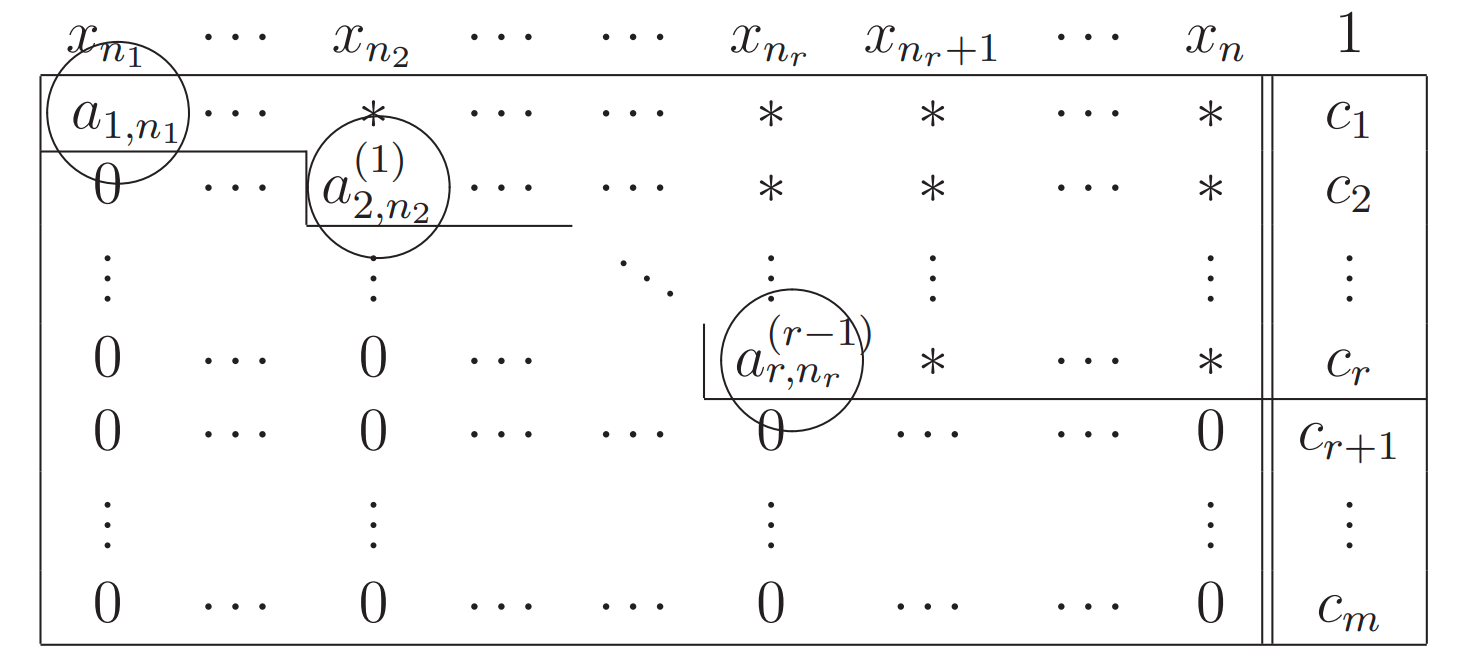
\includegraphics[width=\linewidth]{gauss.png}
\end{center}

\textbf{Verträglichkeitsbedingungen (VTB):} Falls die Verträglichkeitsbedingungen $c_{r+1} = \cdots = c_m = 0$ nicht erfüllt sind, so gibt es keine Lösung. Bei homogenen LGS sind die Verträglichkeitsbedingungen immer erfüllt. Nur wenn $r < n$ gibt es also nicht-triviale Lösungen.\\

\begin{subbox}{Lösungen}
  $Ax = b$ hat mindestens eine Lösung gdw. ($r = m$) oder ($r < m$ und VTB sind erfüllt). In diesem Fall gibt es 1 Lösung falls $r = n$, andernfalls eine $n - r$ Schar an Lösungen.
  \begin{itemize}
    \item $r = m$: $\begin{cases}
      r = m = n\text{: eindeutige Lösung, regulär}\\
      r < n\text{: }\infty\text{ Lösungen mit } n - r \text{ freien Variablen}
    \end{cases}$\\
    \item $r < m$: $\begin{cases}
      r = n\text{: eindeutige Lösung}\\
      r < n\text{: }\infty\text{ Lösungen mit } n - r \text{ freien Variablen}
    \end{cases}$
  \end{itemize}
\end{subbox}

Es gilt immer $r \leq \min(m, n)$.

\section{Matrizen \& Vektoren}

Eine $m \times n$ Matrix hat $m$ Zeilen und $n$ Spalten wobei das $i,j$ Element mit $a_{i,j}$ oder $(A)_{i,j}$ bezeichnet wird. Ein $m \times 1$ Vektor ist ein \textbf{Spaltenvektor} und ein $1 \times n$ Vektor ist ein \textbf{Zeilenvektor} (n-Tupel). Die Elemente $a_{jj}, j = 1,2,\cdots,\min(m,n)$ heissen \textbf{Diagonalelemente}. Für eine \textbf{Diagonalmatrix} $A$ gilt $(A)_{ij} = 0$ für $i = j$. Wir bezeichnen die Matrix dann durch die Elemente auf der Diagonale: $A = diag(d_{11}, \cdots, d_{nn})$. Für eine \textbf{obere Dreiecksmatrix} gilt: $(R)_{ij} = 0$ für $i > j$. Für eine \textbf{untere Dreiecksmatrix} gilt: $(L)_{ij} = 0$ für $i < j$.

\begin{subbox}{Multiplikation}
  Für eine $m \times n$ Matrix $A$ und eine $n \times p$ Matrix $B$ gilt $(AB)_{ij} = \sumn a_{ik} b_{kj}$ wobei $AB$ eine $m \times p$ Matrix ist. Generell \textbf{nicht kommutativ}.
\end{subbox}

\begin{subbox}{}
  $(\alpha \beta)A = \alpha(\beta A)$,
  $(\alpha A)B = \alpha(AB) = A(\alpha B)$,
  $(\alpha + \beta)A = \alpha A + \beta A$,
  $\alpha(A + B) = \alpha A + \alpha B$,
  $A + B = B + A$,
  $A + (B + C) = (A + B) + C$,
  $(AB)C = A(BC)$,
  $(A + B)C = AC + BC$,
  $A(B + C) = AB + AC$
\end{subbox}

Eine \textbf{Linearkombination} der Vektoren $a_1, \cdots, a_n$ ist $\alpha_1 a_1 + \cdots + \alpha_n a_n$.\\
Falls $AB = 0$, so sind $A$ und $B$ \textbf{Nullteiler}.\\
\begin{subbox}{}
  \textbf{Transponiert}: $A^T$ wird definiert als $(A^T)_{ij} = (A)_{ji}$.\\
  \textbf{Hermitesch}: $A^H = (\overbar{A})^T = \overbar{A^T}$.
\end{subbox}
Eine Matrix ist \textbf{symmetrisch} falls $A^T = A$ und hermitesch falls $A^H = A$ (Diagonale reell). \textbf{Schiefsymmetrisch} ist sie falls $A^T = -A$. $AB$ ist genau dann symmetrisch falls $AB = BA$, $A^T A$ und $A A^T$ sind  immer symmetrisch.
\begin{subbox}{}
  $(A^T)^T = A$, $(A^H)^H = A$, $(\alpha A)^T = \alpha A^T$, $(\alpha A)^H = \overbar{\alpha} A^H$, $(A + B)^T = A^T + B^T$, $(A + B)^H = A^H + B^H$, $(AB)^T = B^T A^T$, $(AB)^H = B^H A^H$
\end{subbox}

TODO: Korollar 2.8, Satz 2.4, Rank-Nullity Theorem, matrix orthogonal iff. column vectors are all orthonormal

\begin{subbox}{}
  Seien $A := \begin{psmallmatrix} a_1 & a_2 & \cdots & a_n \end{psmallmatrix} \in \mathbb{E}^{m \times n}, B := \begin{psmallmatrix} b_1 & b_2 & \cdots & b_n \end{psmallmatrix} \in \mathbb{E}^{n \times n}$. Dann gilt $AB = \begin{psmallmatrix} \sum_{i=1}^n b_{i1} a_i & \sum_{i=1}^n b_{i2} a_i & \cdots & \sum_{i=1}^n b_{in} a_i \end{psmallmatrix} \in \mathbb{E}^{m \times n}$.
\end{subbox}

Falls 
$A := \begin{psmallmatrix}
  a_1 & a_2 & \cdots & a_n\\
\end{psmallmatrix} \in \R^{m \times n}, B := \begin{psmallmatrix}
  b_1^\top \\
  b_2^\top \\
  \vdots \\
  b_n^\top
\end{psmallmatrix} \in \R^{n \times k}$, dann gilt $AB = \sum_{i=0}^n a_k b_k^\top$.

\section{Vektorräume}

Zwei Unterräume $U, W \subseteq V$ heissen \textbf{komplementär} falls jedes $x \in V$ eine eindeutige Darstellung $x = u + w$ mit $u \in U$ und $w \in W$ hat ($V$ ist dann direkte Summe von $U$ und $W$). Man schreibt $V = U \oplus W$. Falls zwei Unterräume komplementär sind, folgt $U \cap W = \{0_V\}$.

Falls  $f: U \rightarrow V$ und $g: V \rightarrow W$ lineare Abbildungen zwischen Vektorräumen sind so dass $ g \circ f$ ein Isomorphismus ist, dann gilt $V = \operatorname{Im}f \oplus \operatorname{Ker} g$.

Eine Menge von paarweise orthogonalen Vektoren ist linear unabhängig wenn alle Vektoren ungleich null sind.

\section{Vektorräume mit Skalarprodukt}

\begin{subbox}{Norm}
  Norm in Vektorraum $V$ über $\mathbb{E}$ ist eine Funktion $\lVert \cdot \rVert: V \mapsto \mathbb{R}$ mit:
  \begin{itemize}
    \item positiv definit: $\forall x \in V$, $\lVert x \rVert \geq 0$ und $\lVert x \rVert = 0 \Leftrightarrow x = 0$
    \item homogen: $\lVert \alpha x \rVert = \lvert \alpha \rvert \cdot \lVert x \rVert$ $\forall x \in V, \forall \alpha \in \mathbb{E}$
    \item Dreiecksungleichung: $\lVert x + y \rVert \leq \lVert x \rVert + \lVert y \rVert$ $\forall x, y \in V$
  \end{itemize}
  Ein Vektorraum mit einer Norm heisst normierter Vektorraum.
\end{subbox}

\begin{subbox}{Skalarprodukt}
  Skalarprodukt in einem Vektorraum $V$ über $\mathbb{E}$ ist eine Funktion $\langle \cdot, \cdot \rangle : V \times V \mapsto \mathbb{E}$ mit folgenden Eigenschaften:
  \begin{itemize}
    \item Linear im zweiten Faktor: $\langle x, y + z \rangle = \langle x, y \rangle + \langle x, z \rangle$ und $\langle x, \alpha y \rangle = \alpha \langle x, y \rangle$. Für reelle Skalare auch linear im ersten Faktor.
    \item  Symmetrisch wenn $\mathbb{E} = \mathbb{R}$ und hermitesch wenn $\mathbb{E} = \mathbb{C}$: $\langle x, y \rangle = \overbar{\langle y, x \rangle}$
    \item Positiv definit: $\forall x \in V$, $\langle x, x \rangle \in \mathbb{R}$ (auch für komplexe Vektorräume!), $\langle x, x \rangle \geq 0$, $\langle x, x \rangle = 0 \Leftrightarrow x = 0$
  \end{itemize}
  Falls $\mathbb{E} = \mathbb{C}$, nennt man $V$ auch einen unitären Vekotrraum, für $\mathbb{E} = \mathbb{R}$ auch euklidischer oder orthogonaler Vektorraum.
\end{subbox}

\begin{subbox}{Euklidisches Skalarprodukt}
  $$\langle x, y \rangle := x^Ty$$
\end{subbox}

Orthogonale Matrizen sind für euklidische Normen längentreu, denn $\langle Qx, Qy \rangle = x^\top Q^\top Q y = x^\top y$.

\begin{subbox}{Euklidisches Skalarprodukt}
  $$\langle x, y \rangle := x^Ty$$
\end{subbox}

\begin{subbox}{Euklidische 2-Norm}
  $$\lVert x \rVert_2 = \sqrt[]{x^T x}$$
\end{subbox}

\begin{subbox}{Skalarprodukte über $\R^n$}
  $\langle x, y \rangle$ ist ein Skalarprodukt über $\R^n$ genau dann wenn $\langle x, y \rangle = x^T A y$ wobei $A$ eine symmetrische Matrix mit strikt positiven Eigenwerten ist (positiv-definit).
\end{subbox}

\begin{mainbox}{Cauchy-Schwarz}
  Sei $V$ ein Vektorraum über $\mathbb{E}$ mit Skalarprodukt.
  $$| \langle x, y \rangle | ^2 \leq \langle x, x \rangle \langle y, y \rangle$$
  Das Gleichheitszeichen gilt genau dann wenn $x$ und $y$ linear abhängig sind.
\end{mainbox}

\begin{subbox}{Winkel}
  Seien $x, y, \in V$. Der Winkel zwischen $x$ und $y$ ist gegeben als:
  $$\varphi := \arccos \frac{Re \langle x, y \rangle}{\lVert x \rVert \lVert y \rVert}$$
\end{subbox}

\begin{mainbox}{Parsevalsche Formel}
  Seien $x, y \in V$, $\{ b_1, \cdots, b_n \}$ eine Orthonormalbasis, so dass $\xi_k := \langle b_k, x \rangle$ und $\eta_k := \langle b_k, y \rangle$. Für $k = 1, \cdots, n$ sind $\xi_k$ und $\eta_k$ die Koordinatenvektoren. 

  $$\langle x, y \rangle = \Sigma_{k=1}^n \overbar{\xi_k} \eta_k = \xi^H \eta = \langle \xi, \eta \rangle$$

\end{mainbox}

\begin{subbox}{Orthogonales Komplement}
  Für einen Unterraum $U$ von $V$ ist $U^\bot := \{ y \in V | \{y\} \bot U \}$ das orthogonale Komplement. $U$ und $U^\bot$ sind komplementäre Unterräume in direkter Summe zu $V$.
\end{subbox}

\textbf{Satz 6.3:} A set $M$ of pairwise orthogonal vectors is linearly independent if $O \notin M$.

TODO: positiv definit von ana2 summary

\section{Determinanten}

TODO: Satz 8.12

\section{Eigenwerte}

\begin{subbox}{Eigenschaften von Eigenwerten und Eigenvektoren}
  Für jede Matrix $A \in \mathbb{E}^{n \times n}$ gilt:
  $$\det(A) = \prod_{i=1}^{n} \lambda_i$$
  $$\Tr(A) = \Sigma_{i=1}^n \lambda_i$$
\end{subbox}

TODO: last chapoter, cahpter 10 missing in summary danny

\section{Tabellen}

\begin{mainbox}{Wichtige Werte}
  \begin{center} 
   \begin{tabular}{c|cccccc}
    deg & 0° & 30° & 45° & 60° & 90° & 180° \\
    \midrule
    rad & 0 & $\frac{\pi}{6}$ & $\frac{\pi}{4}$ & $\frac{\pi}{3}$ & $\frac{\pi}{2}$ & $\pi$ \\
    cos & 1 & $\frac{\sqrt{3}}{2}$ & $\frac{\sqrt{2}}{2}$ & $\frac{1}{2}$ & 0 & -1 \\
    sin & 0 & $\frac{1}{2}$ & $\frac{\sqrt{2}}{2}$ & $\frac{\sqrt{3}}{2}$ & 1 & 0 \\
    tan & 0 & $\frac{1}{\sqrt{3}}$ & 1 & $\sqrt{3}$ & $+\infty$ & 0 \\
   \end{tabular}
  \end{center}
\end{mainbox}

\begin{center}
  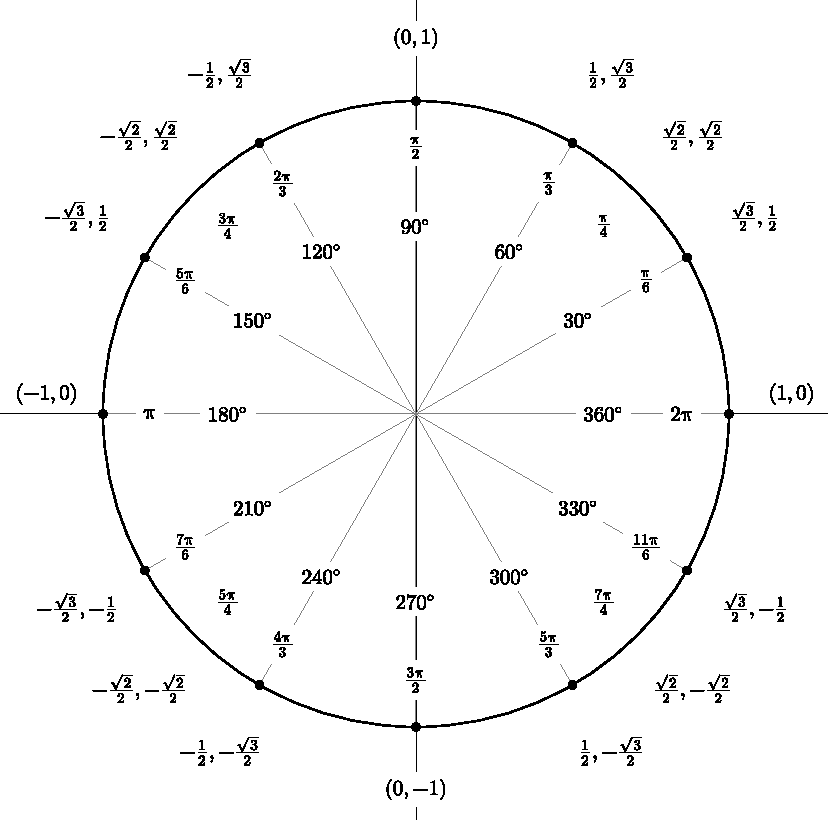
\includegraphics[width=\linewidth]{degrees_circle.pdf}
\end{center}

\end{document}
